\subsection{Planificación de trayectorias}
\label{planificacion}

La planificación de trayectorias toma como entrada toda la información obtenida a través del algoritmo de procesamiento de imágenes: el mapa del entorno, la posición inicial del robot y la posición del objetivo, la lata.\\

El algoritmo elegido para la planificación de la ruta es un Quasi-Randomized Probabilistic Roadmap (Q-PRM), una variante del PRM que utiliza una distribución cuasi-aleatoria de puntos para calcular la hoja de ruta.\\

El algoritmo PRM tiene dos fases principales. En la primera, se genera el PRM propiamente dicho mediante un muestreo del espacio libre a través de una distribución aleatoria de puntos, que se conectan siguendo un criterio de distancias, procurando siempre que , tanto los nodos generados como las aristas que los conectan se encuentren en el espacio libre (no exista colisión con obstáculos. En la segunda, se realizan peticiones de caminos al mapa, conectando un punto inicial y uno final al grafo y calculando el camino más corto mediante un algoritmo de búsqueda en grafos, tal como el Djisktra o el $A^*$.\\

La mejora introducida por la variante Q-PRM es el uso de una distribución de puntos cuasi-aleatoria en lugar de aleatoria, lo que permite elegir una distribución de puntos que rellene el espacio de forma más óptima, siguiendo unos criterios de discrepancia y dispersión. \\

La discrepancia para un conjunto P formado por N muestras de d-dimensiones en $[0,1]^{d}$  viene dada por la ecuación \ref{eq:discrepancia}:
\begin{equation}
\label{eq:discrepancia}
D_N(P) = \sup_{j}{\left| \frac{A(J)}{N} -  \mu(J) \right| }
\end{equation}~\\

Donde J es cualquier subconjunto n-rectangular perteneciente a $[0,1]^{d}$, $\mu(J)$ es su medida n-dimensional y A(J) es el número de puntos que pertenecen a la unión entre P y J. En cuanto a la dispersión, hace referencia a la máxima distancia a la que cada punto de un conjunto puede estar respecto al punto mas cercano perteneciente a la misma secuencia. Por lo general, los conjuntos de puntos que presentan una baja discrepancia también poseerán una baja dispersión.\\

Estas distribuciones de puntos tienen la ventaja de ocupar el espacio libre de forma más eficiente, por lo que con menos cantidad de puntos se puede abarcar un área mayor y, por tanto, más partes delicadas del mapa. Estas partes delicadas pueden ser, por ejemplo, estrechamientos del espacio libre entre obstáculos.\\


Para el muestreo de puntos cuasi-aleatorios se han usado dos distribuciones de puntos: el conjunto de Hammersley y el conjunto de Halton. Estas distribuciones se generan a partir de una semilla para un número arbitrario de dimensiones. Estas distribuciones se pueden calcular de la siguiente manera:
\begin{itemize}
\item \textbf{Conjunto de Hammersley}: Dados $d-1$ números primos distintos $p_1, p_2, ... , p_{d-1}$ el i-ésimo punto del conjunto es dado por la expresión:
\[ \left( \frac{i}{N}, r_{p_1}(i), ..., r_{p_{d-1}(i)} \right), \qquad i = 0, 1, ..., N-1\]

\item \textbf{Conjunto de Halton} Dados $d$ números primos distintos $p_1, p_2, ..., p_d$ el i-ésimo punto del conjunto es dado por la siguiente expresión:
\[ \left( r_{p_1}(i),  r_{p_2}(i), ...,  r_{p_d}(i) \right) \]

\end{itemize}~\\

En ambos casos, la función $r_p(i)$ se obtiene  escribiendo los dígitos de la notación basada en $p$ en orden inverso. Por ejemplo, para la expresión $i = a_0 + a_1 p + a_2 p^2 + a_3 p^3 + ... $ donde $a_j \in \left\lbrace 0, 1, ... , p-1 \right\rbrace$ la función $r_p(i)$ sería:\\

\[ r_p(i) = \frac{a_0}{p} + \frac{a_1}{p^2} + \frac{a_2}{p^3} + \frac{a_3}{p^4} + ...\]\\

La figura \ref{fig:muestreo} muestra una comparativa de los distintos métodos de generación de puntos de muestreo sobre el escenario del CEABOT usado como entorno de trabajo. \\

\begin{figure}[h]
		\centering
        \begin{subfigure}[b]{0.3\textwidth}
                \centering
                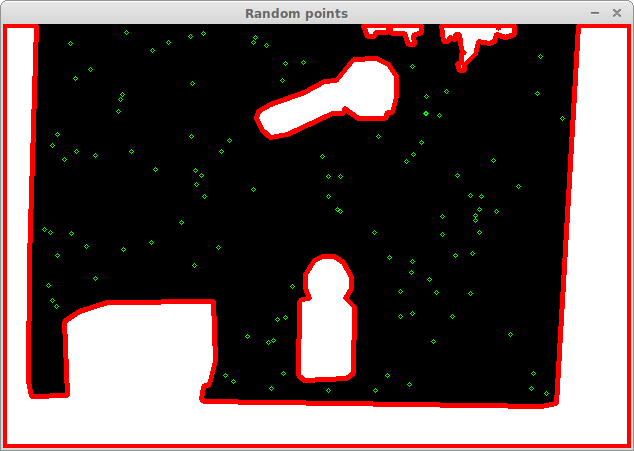
\includegraphics[width=\textwidth]{images/random-beer.png}
                \caption{Muestreo aleatorio}
                \label{fig:muestreo_aleatorio}
        \end{subfigure}
        ~
        \begin{subfigure}[b]{0.3\textwidth}
                \centering
                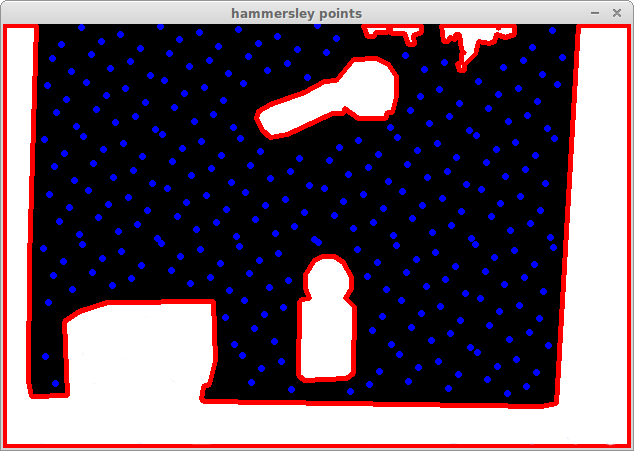
\includegraphics[width=\textwidth]{images/hammersley-beer.png}
                \caption{Muestreo con puntos Hammersley}
                \label{fig:muestreo_hammersley}
        \end{subfigure}
        ~
        \begin{subfigure}[b]{0.3\textwidth}
         	   \centering
                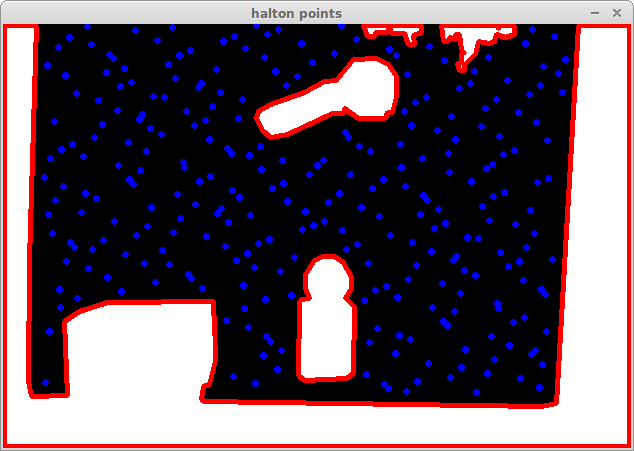
\includegraphics[width=\textwidth]{images/halton-beer.png}
                \caption{Muestreo con puntos Halton}
                \label{fig:muestreo_halton}
        \end{subfigure}
        \caption{Comparativa de los distintos modos de muestreo del espacio libre}\label{fig:muestreo}
\end{figure}

La distribución elegida fue la de Hammersley (figura \ref{fig:muestreo_hammersley}), debido a una mayor dispersión, de forma que la conectividad de la hoja de ruta era mayor.\\

Una vez generados los puntos para el muestreo del espacio libre, se comprueba cada uno de los puntos comprobando colisiones con los obstáculos. Para ello se utiliza un detector de colisiones basado en convolución: para reducir el tiempo de cómputo de colisiones con el modelo del robot, se aplica primero la convolución del círculo que representa al robot sobre toda la imagen, de forma que los obstáculos se dilatan. De esta forma se puede usar la detección de colisión simple, mucho más rápida, sobre los obstáculos dilatados.\\

Tras eliminar los nodos que colisionan con obstáculos, se prodece a la conexión de los distintos nodos para la generación del grafo de la hoja de ruta. El criterio seguido para conectar dos nodos es su vecindad. Se consideran vecinos dos nodos que estén a una distancia entre ellos menor que un valor umbral. Para cada pareja de nodos se calcula la distancia y se coloca en una matriz que reprensenta la conectividad del grafo, y que es usada como entrada de un algoritmo de búsqueda en grafos como Djisktra o $A^*$. Al ser la distancia del nodo A al nodo B la misma que la del nodo B al nodo A, sólo se calculan las distancias una vez.\\

Por último, y antes de añadir cada conexión a la hoja de ruta, se comprueba si esa arista del grafo es una trayectoria válida para el robot o colisiona con algún obstáculo, y sólo se añade en caso de que sea válida. Para la comprobación de la arista, se discretiza en diversos puntos, y se comprueba cada uno de ellos con alguno de los métodos presentados anteriormente. La hoja de ruta resultante se muestra en la figura \ref{fig:hoja_ruta}\\

\begin{figure}[H]
        \centering
        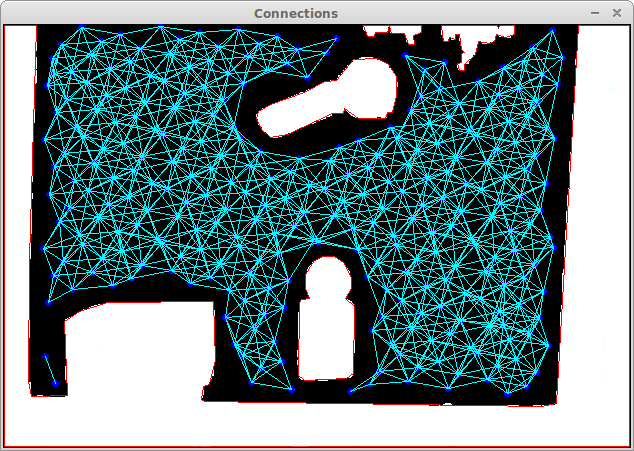
\includegraphics[width=0.5\textwidth]{images/roadmap.png}
        \caption{Hoja de ruta resultante sobre un mapa real extraído del escenario.}
        \label{fig:hoja_ruta}
\end{figure} 

Una vez se ha muestreado el espacio libre y se han conectado los nodos entre si para generar un grafo, el siguiente paso es buscar el camino más corto. Para ello nuestra librería \textit{PLATANO} \footnote{https://github.com/JavierIH/platano} se dispone de dos algoritmos diferentes, el $A^*$ y el Dijkstra.\\

El algoritmo de Dijkstra es un método para encontrar el camino mas corto desde un nodo hasta todos los demás nodos de un grafo, aunque se suele usar para encontrar el camino más corto entre dos nodos, que detine el algoritmo cuando se ha encontrado ese camino. En este algoritmo, el coste de cada nodo (tambien llamado prioridad) se calcula como la distancia entre éste y el nodo inicial, manteniendo una lista de nodos visitados y una de nodos por visitar. De esta forma se recorre el grafo viajando siempre por los nodos de menor distancia hasta que se encuentra un nodo anterior con menor distancia o se llega hasta el nodo objetivo. y revisar \\

El algoritmo $A^*$, una evolución del algoritmo de Dijkstra, busca devolver la trayectoria que vaya del nodo inicial al final y que presente un coste más bajo. Mientras va explorando un camino mantiene otras posibles soluciones para cambiar de trayectoria, en caso de que la que se está recorriendo deje de ser óptima. Este algoritmo garantiza que siempre se encontrará una solución, si existe alguna.\\

El coste que se emplea para comparar las distintas posibles trayectorias entre sí viene dado por la suma de dos funciones. La primera es la distancia recorrida entre el nodo inicial y el nodo para el cual se está calculando el coste, mientras que la segunda consiste en una estimación de la distancia que es necesario recorrer para llegar al punto de destino. Aunque esto último se puede representar de diversas maneras, lo mas común es calcular la distancia en linea recta desde el nodo actual hasta el final.\\

Una vez obtenida la trayectoria como una secuencia de puntos por los que el robot debe pasar hasta llegar a la meta, estos puntos son pasados al controlador del robot para que realice el movimiento hasta la lata.\\